\documentclass[10pt,twoside]{article}
\usepackage{graphicx}
\usepackage{url}

\newcommand{\doctitle}{%
Sudoku Solver}
\newcommand{\cmnt}[1]{}
\newcommand{\sps}{State Space Search}

\pagestyle{myheadings}
\markboth{\hfill\doctitle}{\doctitle\hfill}

\bibliographystyle{siam}

\addtolength{\textwidth}{1.00in}
\addtolength{\textheight}{1.00in}
\addtolength{\evensidemargin}{-1.00in}
\addtolength{\oddsidemargin}{-0.00in}
\addtolength{\topmargin}{-.50in}

\hyphenation{in-de-pen-dent}

%\title{\textbf{\doctitle}\\
\title{\textbf{ CS598 Project Proposal: Parallel Sudoku Solver}}

\author{Sandeep Dasgupta\thanks{Electronic address: \texttt{sdasgup3@illinois.edu}}
\qquad Tanmay Gangwani\thanks{Electronic address: \texttt{gangwan2@illinois.edu}}
\qquad  Mengjia Yan\thanks{Electronic address:
\texttt{myan8@illinois.edu}}} 

\begin{document}

\thispagestyle{empty}

\maketitle
  \sps is vividly used in modelling problems in artificial intelligence, planning and optimization literature, where
  the set of states forms a graph where two states are connected if there is an operation that can be performed to transform the first state into the second.
  A typical \sps consists of many states to explore which imposes serious
  contraints on the exploration time and memory. Given the exponential amount
  of work that \sps problems entail, it is desirable to solve
  them on large parallel machines with significant computational power. 

  Challenges to parallel \sps \\
  Parallel implementation of this search procedure requires the distribution of
  work into discrete chunks or tasks. To ensure the efficient execution of
  these tasks on processors, the inter-related issues of task creation,
        grainsize control, and load balance must be considered. 
  \begin{itemize}        
    \item
          Grainsize can
          be defined roughly as the ratio of computation work to number of
          messages sent. This can be decided by a careful formulation od a
          metric correlated to the computation cost of a node. With a suitable
          metric formulated, a threshold amount of work may be set, below which
          new tasks are not created; such subtrees are explored sequentially.
     \item  
          Moreover there is a certain overhead in creating tasks, and a separate
          overhead if the task description is moved to another processor. Thus,
        it is important to keep the average grainsize above a certain threshold
          to limit the impact of parallel overhead. At the same time, no single
          task should be so large as to make all processors wait for its
          completion.

     \item
  Variable Selection:
  Given a particular node in the search tree, there is a choice of which branch to select when consid-
ering new children. This is called variable selection.
  A good heuristic is to select the most constrained variable at each step.
  \end{itemize}

Brief Ideas \\ 
  1. In our project we will start with   parallelizing the graph coloring problem,  searching for any 
  Feasible solution out of the corresponding \sps.  
  One of the many challenges is ``Value ordering'' which is going to play an improtant role : given b children of a node, explore the subtree of that child next whose subtree is
most likely to contain a solution. We will use problem-specific figures of merit   to order the children. 

Also as we know the speculative nature of the methods in this context: regions of the tree that may not be visited in a sequential procedure are
searched concurrently in the hope that a solution may be found quicker. This can lead to anomalies
in parallel performance. We are planning to consistent speedps by adopting the prioritization strategy as emplyed by Kale[].



  Sudoku puzzles consists of partially filled matrix $N \times N$. The algorithm needs
  to fill the blank positions with values 1 through N such that no number is
  repeated on each of the N rows, N columns or the squares of $\sqrt{N} \times
  \sqrt{N} $ cells that split the original matrix.  The goal will be to solve
  the grid in the least possible time using the parallelization model provided by Charm++.

  Sudoku is an NP-complete problem. The solution space rapidly explodes as we move to 
  higher grid dimensions. For example, it has been proven that the total number of
  valid Sudoku grids, for $N = 9$,  is $6,670,903,752,021,072,936,960$ or
  approximately $6.671 \times 10^{21}$. This precludes using brute force techniques. We would 
  investigate heuristics based on the "logical' properties of Sudoku to reduce the search space 
  and optimize the running time of the algorithm. Sudoko solutions are achieved incrementally by 
  solving instances of smaller problems. Updates to one part of the grid may significantly
  impact other parts which leads to a high degree of communication between objects handling the 
  grid. Load imbalance is inherent in the problem since some parts of the grid may be easier to
  proceed with than other. We plan to leverage the Charm++ model to tackle these challenges. In later 
  stages of the project, we may include the use of the Charm checkpointing support for a part of the
  algorithm which guesstimates certain numbers, and backtracks if a dead end is found.

  \begin{figure}[h]
  \centering
    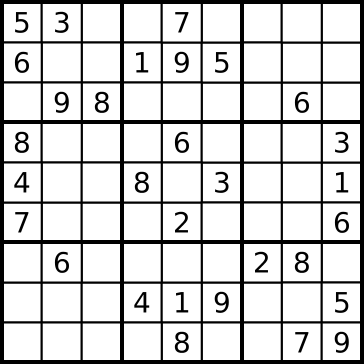
\includegraphics[scale=0.35]{sudoku} 
  \caption{Sudoku Grid} 
  \end{figure}

  




%\nocite{*}
%\bibliography{CS598_project_proposal}

\end{document}
